\section{Value-Based}
\label{section:value-based}
Value-based methods typically aim at finding $Q^*$ first, which then gives the optimal policy $\pi^*(s) = \argmax_a Q^*(s,a)$. For this, they require finite action spaces.
% Like other model-free approaches, the agent needs to interact with the environment to learn.

\subsection{Tabular environments}
In the case of tabular environments (i.e. $S$ is finite as well), $Q^\pi$ can actually be represented by a matrix.

\paragraph{Tabular Q-learning}
Starting from a random value-action function $Q$, tabular Q-learning consists in interacting with the environment and applying equation \ref{eq:bellman-q*} to converge to $Q^*$ (algorithm \ref{algo:tabular-q-learning}). Q-learning is an \emph{off-policy} method, i.e. learns the value of the optimal policy independently of the agent's actions, and $\pi$ can be any policy as long as all state-action pairs are visited enough.

\begin{algorithm}[H]
\DontPrintSemicolon
\For{a number of episodes}{
    initialize $s_0$ \;
    \While{episode not done}{
        take action $a_t \sim \pi(s_t)$, observe $r_t$ and $s_{t+1}$ \;
        $Q(s_t,a_t) \leftarrow Q(s_t,a_t) + \alpha \left[ r_t + \gamma \max_a Q(s_{t+1}, a) \right]$ \;
    }
}
\caption{Tabular Q-learning}
\label{algo:tabular-q-learning}
\end{algorithm}

\paragraph{SARSA} The SARSA algorithm is the \emph{on-policy} equivalent of Q-learning as it learns the value of the current agent's policy $\pi$. Instead of using Bellman equation \ref{eq:bellman-q*}, it uses equation \ref{eq:bellman-q} for the update step, and converges to the optimal policy $\pi^*$ as long as policy $\pi$ becomes greedy in the limit.

\paragraph{Exploration strategies} \label{paragraph:exploration-strategies} Used by value-based algorithms (SARSA, Q-learning) to balance between exploration and exploitation when interacting with the environment.
\begin{itemize}
    \item \emph{$\epsilon$-greedy strategy}
        \[
          \pi(s)=\begin{cases}
            \argmax_a Q(s,a) & \text{be greedy with probability $\epsilon$}\\
            \textit{a random action}, & \text{otherwise}
          \end{cases}
        \]
    \item \emph{Boltzmann selection}
        \[
          \pi(a|s) = \frac{\exp(Q(s,a)/\tau)}{\sum_{a'} \exp(Q(s,a')/\tau)}
        \]
    \item Others: UCB-1, pursuit strategy. Comparison in \cite{tijsma2016comparing} (for stochastic mazes).
\end{itemize}

\paragraph{Temporal Difference (TD) learning} TD methods combine Monte-Carlo (MC) sampling \footnote{Since we don't know the MDP, we have to approximate the expectation using trajectory samples} with the \emph{bootstrapping} of DP methods \footnote{Bootstrapping: using our current approximation of $V^{\pi}(s')$ to estimate $V^{\pi}(s)$}, and are used to learn $V^\pi$ or $Q^\pi$. The following quantity
\[
    \delta_t = r_{t+1} + \gamma V(s_{t+1}) - V(s_t)
\]
is called the \emph{TD-error}.

\begin{itemize}
    \item \emph{TD(0) learning} is the most straightforward method. After acting according to $\pi$, the value function is updated with: 
    \[
        V(s_t) \leftarrow V(s_t) + \alpha [r_t + \gamma V(s_{t+1}) - V(s_t)]
    \]
    Since $\E[r_t + \gamma V^\pi(s_{t+1})] = V^\pi(s_t)$, $V$ will eventually converge to $V^\pi$. 
    % todo: understand the difference with TD(1)
    
    \item \emph{Multi-steps learning}. When the reward is delayed and is observed several steps after the decisive action, TD(0) is slow since values only propagate from one state to the previous one. With:
    \[
        G_t^{(n)} = r_t + \gamma r_{t+1} + \dots + \gamma^{n-1} r_{t+n} + \gamma^n V^\pi(s_{t+n})
    \]
    the \emph{$n$-step return}, it is also true that $\E[G_t^{(n)}] = V^\pi(s_t)$. Therefore, the update steps becomes: 
    \[
        V(s_t) \leftarrow V(s_t) + \alpha [G_t^{(n)} - V(s_t)]
    \]
    Multi-steps learning can converge faster depending on the problem. As $n \rightarrow \infty$, this update approaches the unbiased MC estimate of $V^\pi$, at the cost of higher variance.

    \item \emph{TD($\lambda$) learning}. Instead of choosing the right $n$, a better way to navigate between TD(0) and MC updates is to average all $n$-step returns with a decay $\lambda$. For $\lambda \in [0,1)$, the \emph{$\lambda$-return} is defined as
    \[
        G_t^\lambda = (1-\lambda) \sum_{n=1}^\infty \lambda^{n-1} G_t^{(n)}
    \]
    and also verifies $\E[G_t^\lambda] = V^\pi(s_t)$, therefore can be used in the update step. Choosing $\lambda=0$ is equivalent to TD(0) updates, and $\lambda \rightarrow 1$ approaches MC updates.
\end{itemize}

\paragraph{Eligibility traces} Eligibility traces $e_t$ are an equivalent but more convenient way of implementing TD($\lambda$) learning. Updates are done online (\emph{backward view}) instead of having to wait the end of the trajectory (\emph{forward view}).
% todo: check
% Note: these are actually accumulating traces, but other versions exist (https://www.cs.utexas.edu/~pstone/Courses/394Rfall16/resources/week6-sutton.pdf):
% - dutch traces, equivalent to TD(lambda) and with a sound background (better than accumulating traces?), but can only be implemented with tabular env (?) cf sutton
% - replace traces, a crude approximation to dutch traces

\begin{algorithm}[H]
\DontPrintSemicolon
\For{a number of episodes}{
    initialize $s_0$ and set $e_0(s)=0, \forall s$\;
    \While{episode not done}{
        take action $a_t=\pi(s_t)$, observe $r_t$ and $s_{t+1}$ \;
        \For{all $s$}{
          $e_t(s) \leftarrow \lambda \gamma e_{t-1}(s) + \mathbbm{1}_{s_t=s}$ \tcp*{this leads to $e_t(s) = \sum_{k=0}^t(\lambda \gamma)^{t-k} \mathbbm{1}_{s_k=s}$}
          $V(s_t) \leftarrow V(s_t) + \alpha e_t(s) \delta_t$ \;
        } 
    }
}
\caption{Eligibility traces, also called online TD($\lambda$), tabular version}
\label{algo:eligibility-traces}
\end{algorithm}

\todo{version with weights}

\begin{figure}[H]
    \centering
    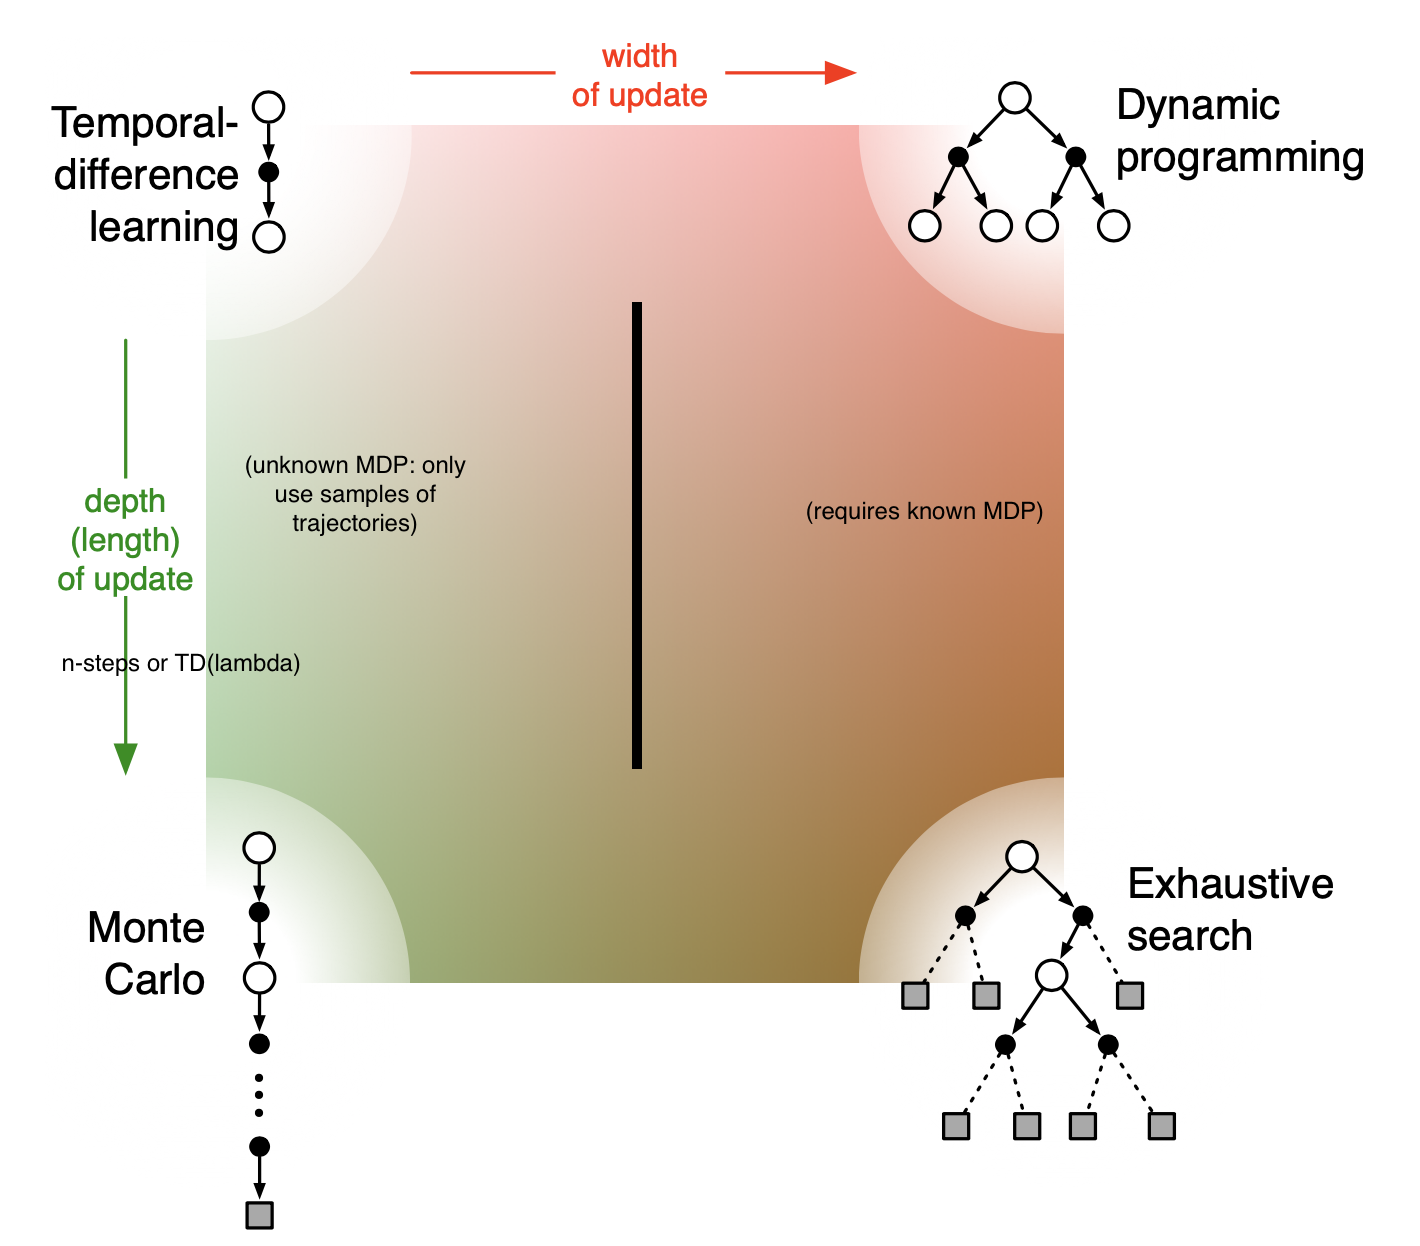
\includegraphics[width=0.5\linewidth]{figures/td-learning.png}
    \caption{Taken from \cite{sutton2018reinforcement}}
    \label{fig:td-learning}
\end{figure}


\subsection{Approximate Q-learning}
Tabular learning approaches have trouble learning in large environments since there is no generalization between similar situations, and storing Q or V can even be an issue. Approximate approaches allow working with large finite environments and even with continuous state space $S$, by considering
\[
    Q(s,a) \approx Q_\theta(\phi(s),a)
\]
with $\phi(s) \in \mathbb{R}^d$ a vector of features. Features $\phi$ can be hand-crafted, but in Deep Reinforcement Learning (DRL) they are typically learned using neural networks and we simply note $Q(s,a) \approx Q_\theta(s,a)$.

\paragraph{Deep Q-Network (DQN) \cite{mnih2013playing}\cite{mnih2015human}} DQN was the first successful attempt at applying DRL on high-dimensional state spaces, and uses 2D convolutions with an MLP to extract features. It overcomes stability issues thanks to:
\begin{itemize}
    \item \emph{Experience-replay}. Within a trajectory, transitions are strongly correlated but gradient descent algorithms typically assume independent samples, otherwise gradient estimates might be biased. Storing transitions and sampling from a memory buffer $D$ reduces correlation, and even allows mini-batch optimization to speed up training. Re-using past transitions also limits the risk of catastrophic forgetting.
    \item \emph{Target network}. Based on eq. \ref{eq:bellman-q*}, values $Q_\theta(s,a)$ can be learned by minimizing the error\footnote{This can be the mean square error, or Huber loss for more stability} to the target $r + \gamma \max_{a'}Q_\theta(s',a')$. In this case, $\theta$ is continuously updated and we are chasing a non-stationary target. Learning can be stabilized by using a separate network $Q_{\theta^-}$ called the target network, with weights $\theta^-$ updated every $k$ steps to match $\theta$.
\end{itemize}

\begin{algorithm}[H]
\DontPrintSemicolon
\SetKwInput{Init}{Init}
\Init{replay memory $D$ with capacity $M$, $Q_\theta$ with random weights, $\theta^- = \theta$}
\For{a number of episodes}{
    initialize $s_0$ \;
    \While{episode not done}{
        take action $a_t \sim \pi(s_t)$, observe $r_t$ and $s_{t+1}$ \tcp*{$\pi$ can be $\epsilon$-greedy for instance}
        store transition $(s_t, a_t, r_t, s_{t+1})$ in $D$ \;
        sample random mini-batch of transitions $\left((s_j, a_j, r_j, s_{j+1})\right)_{j=1,\dots,N}$ from $D$ \;
        set $y_j=\begin{cases}
            r_j & \text{if $s_{j+1}$ is a terminal state}\\
            r_j + \gamma \max_{a'} Q_{\theta^-}(s_{j+1},a') & \text{otherwise}
          \end{cases}$ \;
        $\theta \leftarrow \theta - \alpha \nabla_\theta \frac{1}{N} \sum_{j=1}^N (y_j - Q_\theta(s_j,a_j))^2$ \;
        every $k$ steps, update $\theta^- = \theta$ \;
    }
}
\caption{Deep Q-learning with experience replay and target network (DQN)}
\label{algo:DQN}
\end{algorithm}

\paragraph{Prioritized Experience Replay (PER) \cite{schaul2015prioritized}}
Improve experience replay: rather than sampling transitions $t_i$ uniformly from the memory buffer, prioritize the ones that are the most informative, i.e. with the largest error.
\[
i \sim P(i) = \frac{p_i^\alpha}{\sum_k p_k^\alpha}
\quad \text{with} \quad
p_i = |\delta_i| + \epsilon
\]
And $\delta_t = r_t + \gamma \max_a Q(s_{t+1},a) - Q(s_t, a_t)$ the TD-error again. In practice when implementing PER, errors $\delta_i$ are stored in memory with their associated transition $t_i$ and are only updated with current $Q_\theta$ when $t_i$ is sampled. A SumTree structure can be used to efficiently sample from $P(i)$, in $O(\log |D|)$. Since PER introduces a bias\footnote{This \href{https://danieltakeshi.github.io/2019/07/14/per/}{blog post} goes into more details}, authors use \emph{importance sampling} and correct the loss with a term $w_i = 1 / (N P(i))^\beta$.

\paragraph{Double DQN \cite{van2016deep}}
Because it is using the same value function $Q_\theta$ for both action selection and evaluation in the target $y_t = r_t + \gamma \max_a Q_\theta(s_{t+1}, a)$, Q-learning tends to overestimate action values as soon as there is any estimation error. This is particularly the case when the action space is large (figure \ref{fig:double-dqn}). Double Q-learning \cite{hasselt2010double} decouples action selection and evaluation using 2 parallel networks $Q_\theta$ and $Q_{\theta'}$. Double DQN \cite{van2016deep} improves DQN performance and stability by doing it simply with the online network $Q_\theta$ and target network $Q_{\theta^-}$:
\[
    y_t = r_t + \gamma Q_{\theta^-}(s_{t+1}, \argmax_a Q_\theta(s_{t+1}, a))
\]

\begin{figure}[H]
    \centering
    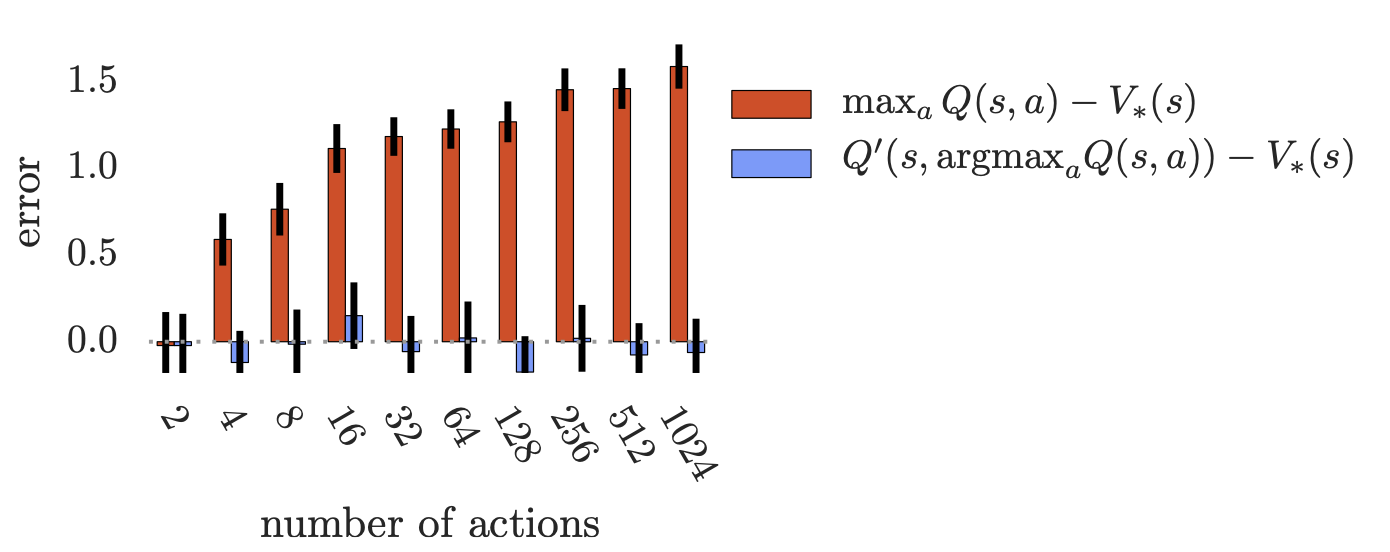
\includegraphics[width=0.5\linewidth]{figures/double-dqn.png}
    \caption{Taken from \cite{van2016deep}}
    \label{fig:double-dqn}
\end{figure}

\paragraph{Rainbow \cite{hessel2018rainbow}}
Rainbow studies and combines a number of improvements to the DQN algorithm: multi-steps returns, prioritized experience replay, Double Q-learning, as well as dueling networks (using a value function $V_\theta(s)$ and an advantage function $A_\theta(s,a)$ to estimate $Q(s,a)$), noisy nets (adaptive exploration by adding noise to the parameters of the last layer, instead of being $\epsilon$-greedy) and distributional RL (approximate the distribution of returns instead of the expected return).

\paragraph{Deep Recurrent Q-Network \cite{hausknecht2015deep}}
By using a RNN to learn the features (e.g. after the convolutional layers), DQRN keeps in memory a representation of the world according to previous observations. This makes it possible to go beyond the Markov property and work with POMDPs, but it can be harder to train.
